\chapter{Basi teoriche}
\label{cap:teoria}
\intro{Per comprendere al meglio gli argomenti trattati nel capitolo successivo è necessaria un'introduzione teorica}

\section{Machine learning}
Il machine learning è un'applicazione della statistica che si concentra sullo sviluppo di algoritmi in grado di imparare dai dati che vengono loro forniti in input.
Da un punto di vista più filosofico il machine learning è interessante perché sviluppando la nostra conoscenza su di esso stiamo di conseguenza migliorando la nostra comprensione dei principi su cui si sorregge l'intelligenza \footcite[p.~97]{Goodfellow-et-al-2016}.
Gli algoritmi di machine learning si suddividono in due categorie principali:

\begin{itemize}
    \item apprendimento supervisionato
    \item apprendimento non supervisionato 
\end{itemize}

\subsection{apprendimento supervisionato}
Gli algoritmi che appartengono a questa categoria apprendono quali risultati generare seguendo la guida di un set di dati etichettati e con un output predefinito\footcite{site:machine-learning}.

\subsection{apprendimento non supervisionato}
Gli algoritmi non supervisionati, anche conosciuti come apprendimento automatico, analizzano e raggruppano dataset non etichettati. Questi algoritmi riconoscono raggruppamenti di dati (cluster) senza la necessità dell'intervento umano\footcite{site:machine-learning}.

\section{K-means}
Il K-means è un algoritmo non supervisionato che viene utilizzato per il clustering, ossia per la suddivisione del dataset in gruppi che contengono caratteristiche simili.
Suddivide un set di dati in gruppi simili sulla base della distanza tra i loro centroidi. 
Il centroide, è la media di tutti i punti presenti all'interno del cluster.

Il numero K sta a indicare quanti cluster dovranno essere assegnati dall'algoritmo, più il numero di cluster è elevato più essi saranno piccoli e dettagliati al contrario se i cluster sono pochi il risultato saranno dei cluster più grandi ma meno dettagliati.

Ad esempio se volessimo clusterizzare un insieme di animali composto da mammiferi e uccelli utilizzando K=2 l'algoritmo creerebbe due cluster uno contenente i mammiferi e uno gli uccelli (cluster grandi e poco dettagliati).
Se aumentassimo il numero di cluster l'algoritmo sarebbe in grado di essere più specifico andando a creare una quantità molto più elevata di cluster ben dettagliati contenenti meno elementi.
Quindi è importante scegliere con cura il numero iniziale K da assegnare, per semplificare questa operazione esistono dei metodi di supporto:
\begin{itemize}
    \item Il metodo del gomito sfrutta l’inerzia, ossia la somma delle distanze al quadrato dei punti dal centroide (SSE, Sum of Squared Errors). Con l'aumento dei cluster, l’inerzia diminuisce, ma dopo un certo punto, la riduzione diventa superflua, venendo a creare una curva a gomito. Il punto in cui la curva si piega indica il numero di cluster da utilizzare.
    
    \begin{figure}[!h] 
        \centering 
        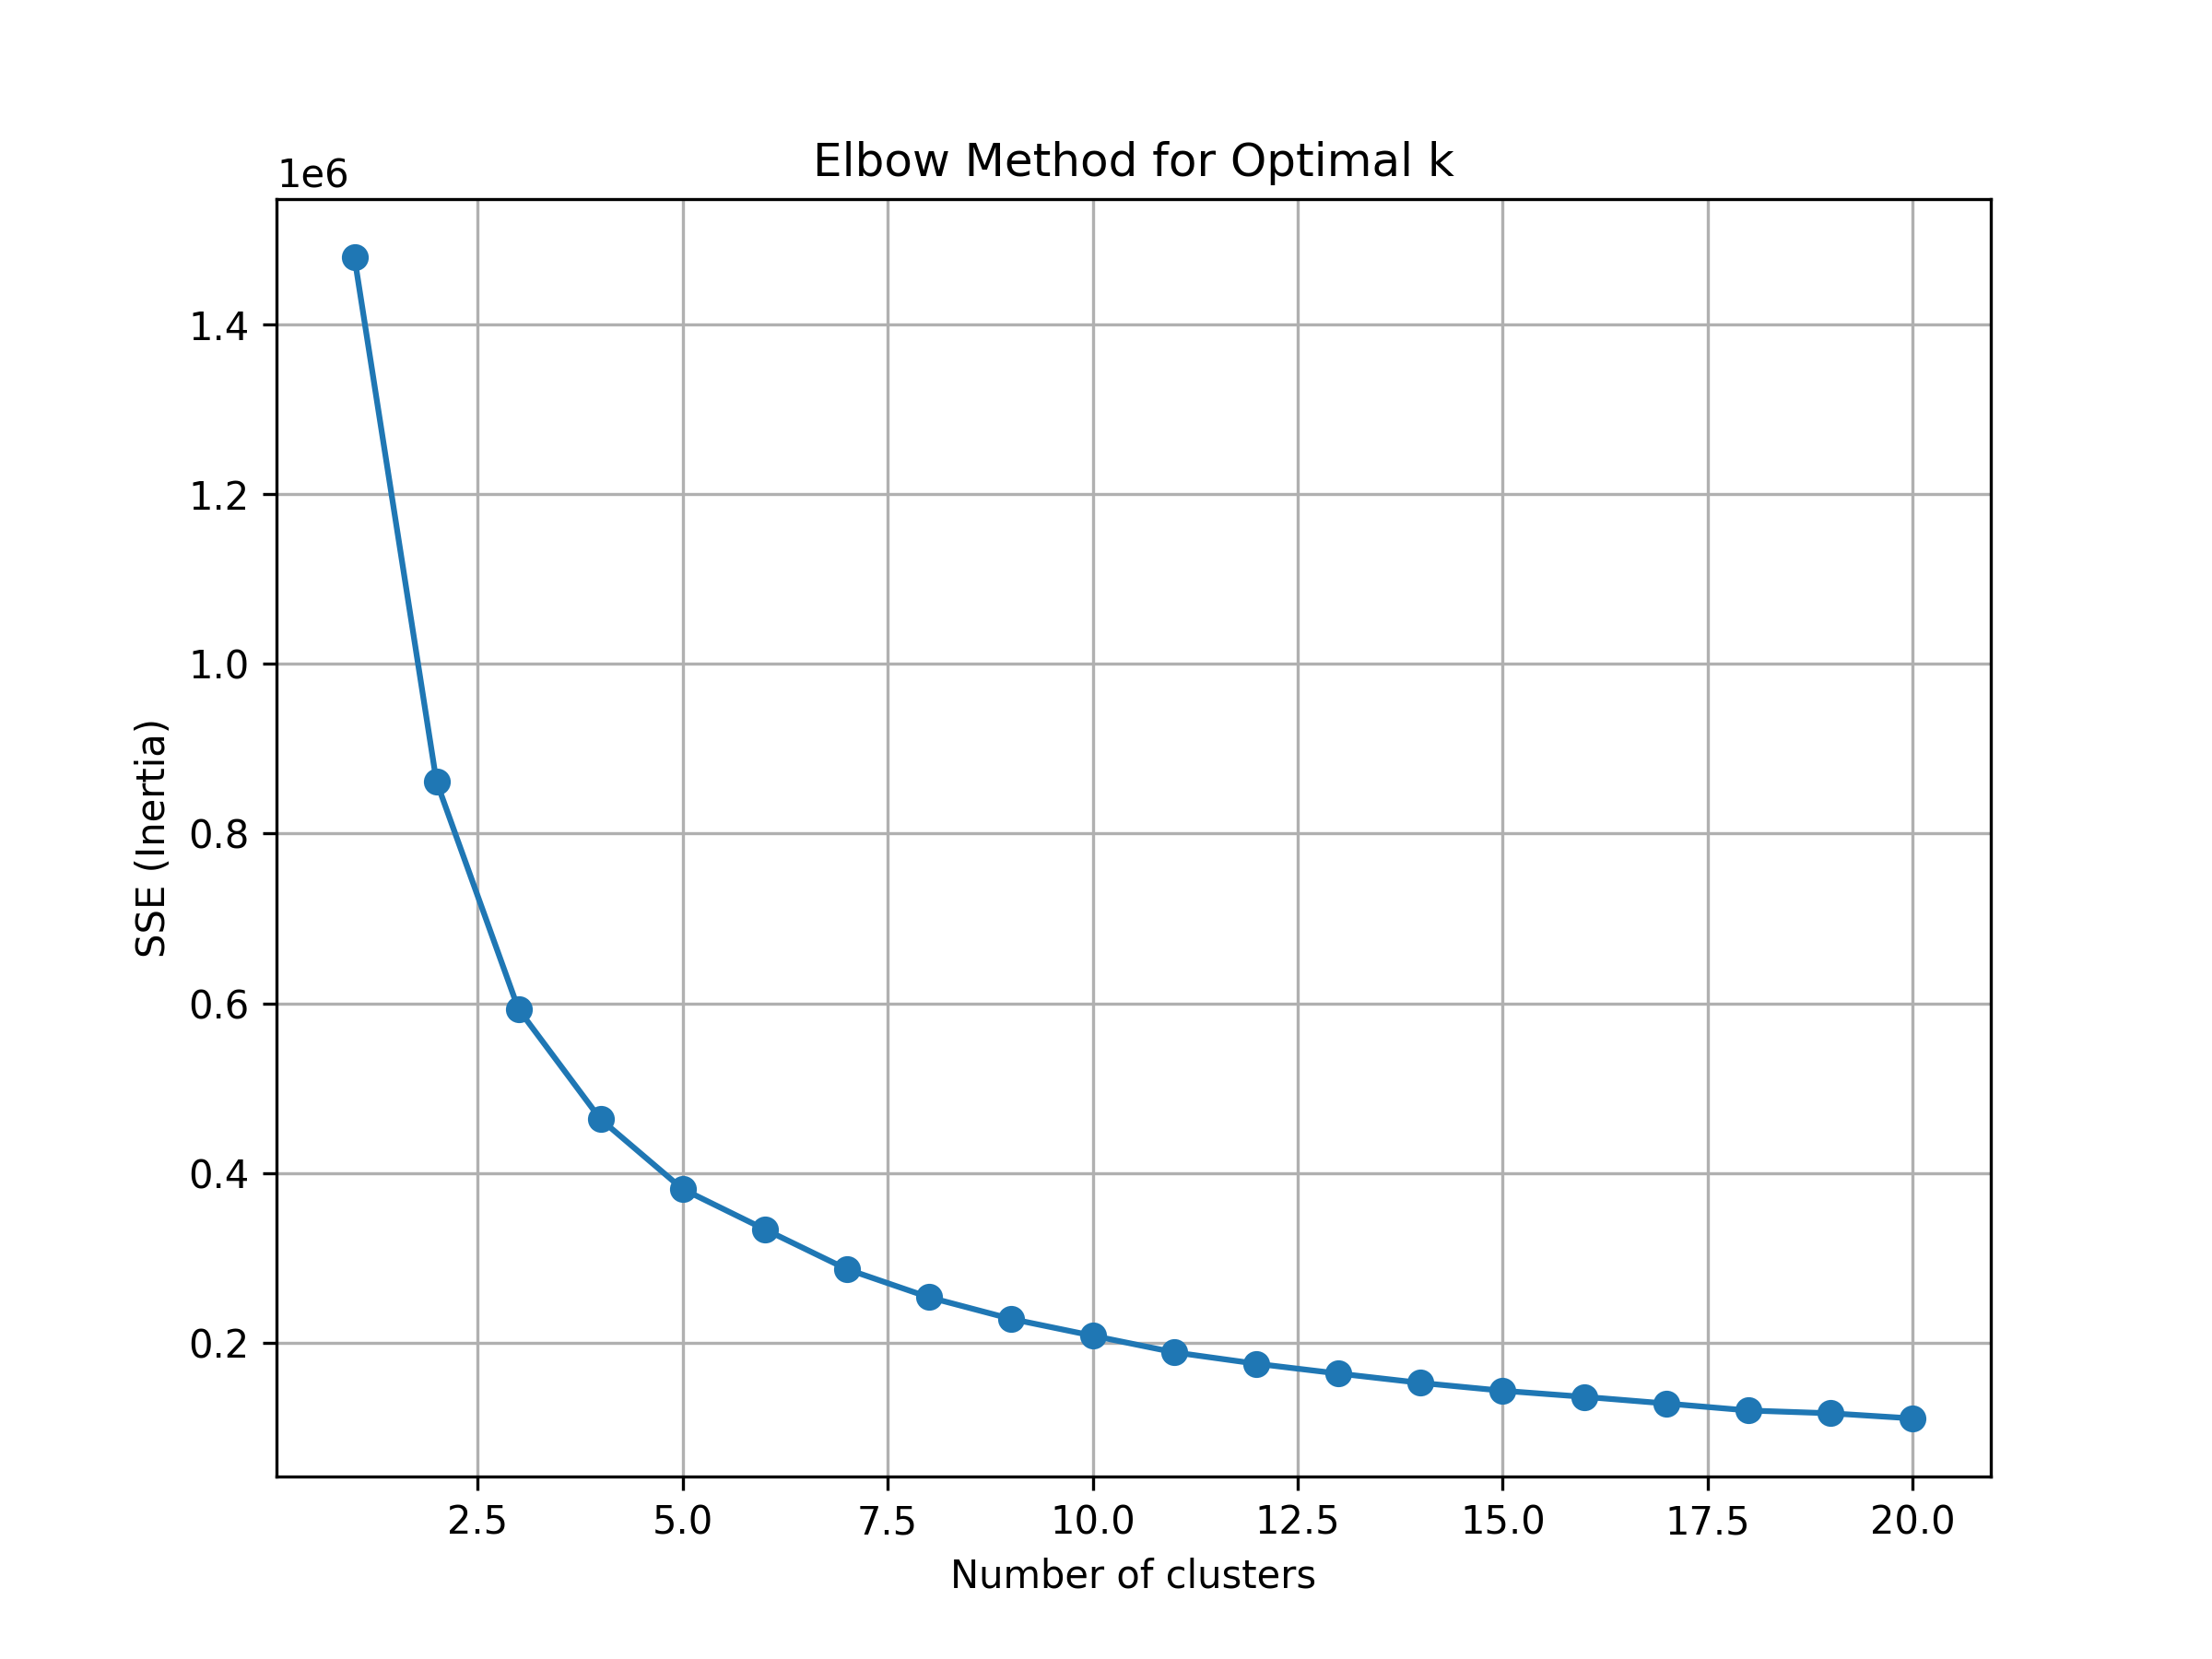
\includegraphics[width=0.7\columnwidth]{teoria/elbow_method.png} 
        \caption{Conversione e ridimensionamento}
        \label{fig:gomito}
      \end{figure}

    \item Il Silhouette Score indica quanto i punti appartenenti a un cluster sono simili tra loro e quanto differiscono dai punti contenuti negli altri cluster.
    Varia tra -1 e 1, se il valore è vicino a 1 il punto è all'interno del suo cluster e ben separato dai cluster limitrofi, se è vicino a 0 il punto è confinante tra due cluster infine un valore negativo indica l'assegnazione a un cluster sbagliato.
\end{itemize}

%dovresti spiegare come funziona realmente ma vediamo che dice il prof

\subsubsection{PCA}
\section{feature}



\section{Deep learning}

\section{CNN}
\subsection{Layer convoluzionali}

\section{Autoencoder}

\section{fine-tuning}


\section{Loss functions}
\section{epoche}
\section{pesi}
\section{activation function}
\section{learning rate}





